%********************************************************************
% Kapitel 4
%*******************************************************
\chapter{Challenges}
\label{ch:Challenges}

\section{Spotify API Limitations}

While the Spotify Web API handles a lot of aspects like authentication with OAuth and retrieving user as well as track data, we have noticed that it comes with certain limitations.

\subsection{Rate Limiting}

Spotify does limit the amount of requests a certain application can do. It is not known, how large the limit is and how long it lasts. The documentation states the following:

\begin{quote}
    If Web API returns status code 429, it means that you have sent too many requests. When this happens, check the Retry-After header, where you will see a number displayed. This is the number of seconds that you need to wait, before you try your request again. \\
    --- Spotify Web API Documentation \cite{SpotifyWebApi}
\end{quote}

To ensure that we do not run into such limit we have decided to cache requests to Spotify. The cache is in-memory and will last for five minutes by default. So if you were wondering why the recently played page does not update immediately, that is why. Using a request cache is advantageous anyways because we do not store any track information in our database but obtain it from Spotify every time we want to display some information in the \ac{UI}. This way we can avoid unnecessary requests to Spotify on page refreshes.

\subsection{Query Size Limits}

Although the Spotify API provides pagination, its maximum page size is limited to 50. This would not be a problem if we could query for a unlimited or at least large amount of pages. Unfortunately, that is not the case. For example, the recently played endpoint defaults to a page size of 20. Querying the first and second pages works as expected and you will get 40 entries. Page three does (surprisingly) return only ten entries though. Looking up the next page will yield no entries so you effectively can not fetch more than 50 entries, even if you change page size to 50 (the second page will be empty in this case).

\subsection{Private \& Beta APIs}

Much to our surprise we did discover that the browser variant of Spotify (\url{https://open.spotify.com}) does not use the same public API that we are using. That is an issue because the public API does not comprise the same feature set as the private API. To demonstrate one of the issues we did encounter we will look at the recently played example again.

\begin{itemize}
    \item Public API: \url{https://api.spotify.com/v1/me/player/recently-played}
    \item Private API: \url{https://api.spotify.com/v1/views/recently-played}
\end{itemize}

While the public API is documented, the private one is not. The latter one does support more pages so you can query much more entries. It also does support querying entries that are not tracks, so you can also query albums, artists or even playlists. The public API does not allow for those same query parameters the private API uses.

\begin{figure}[bth]
    \centering
    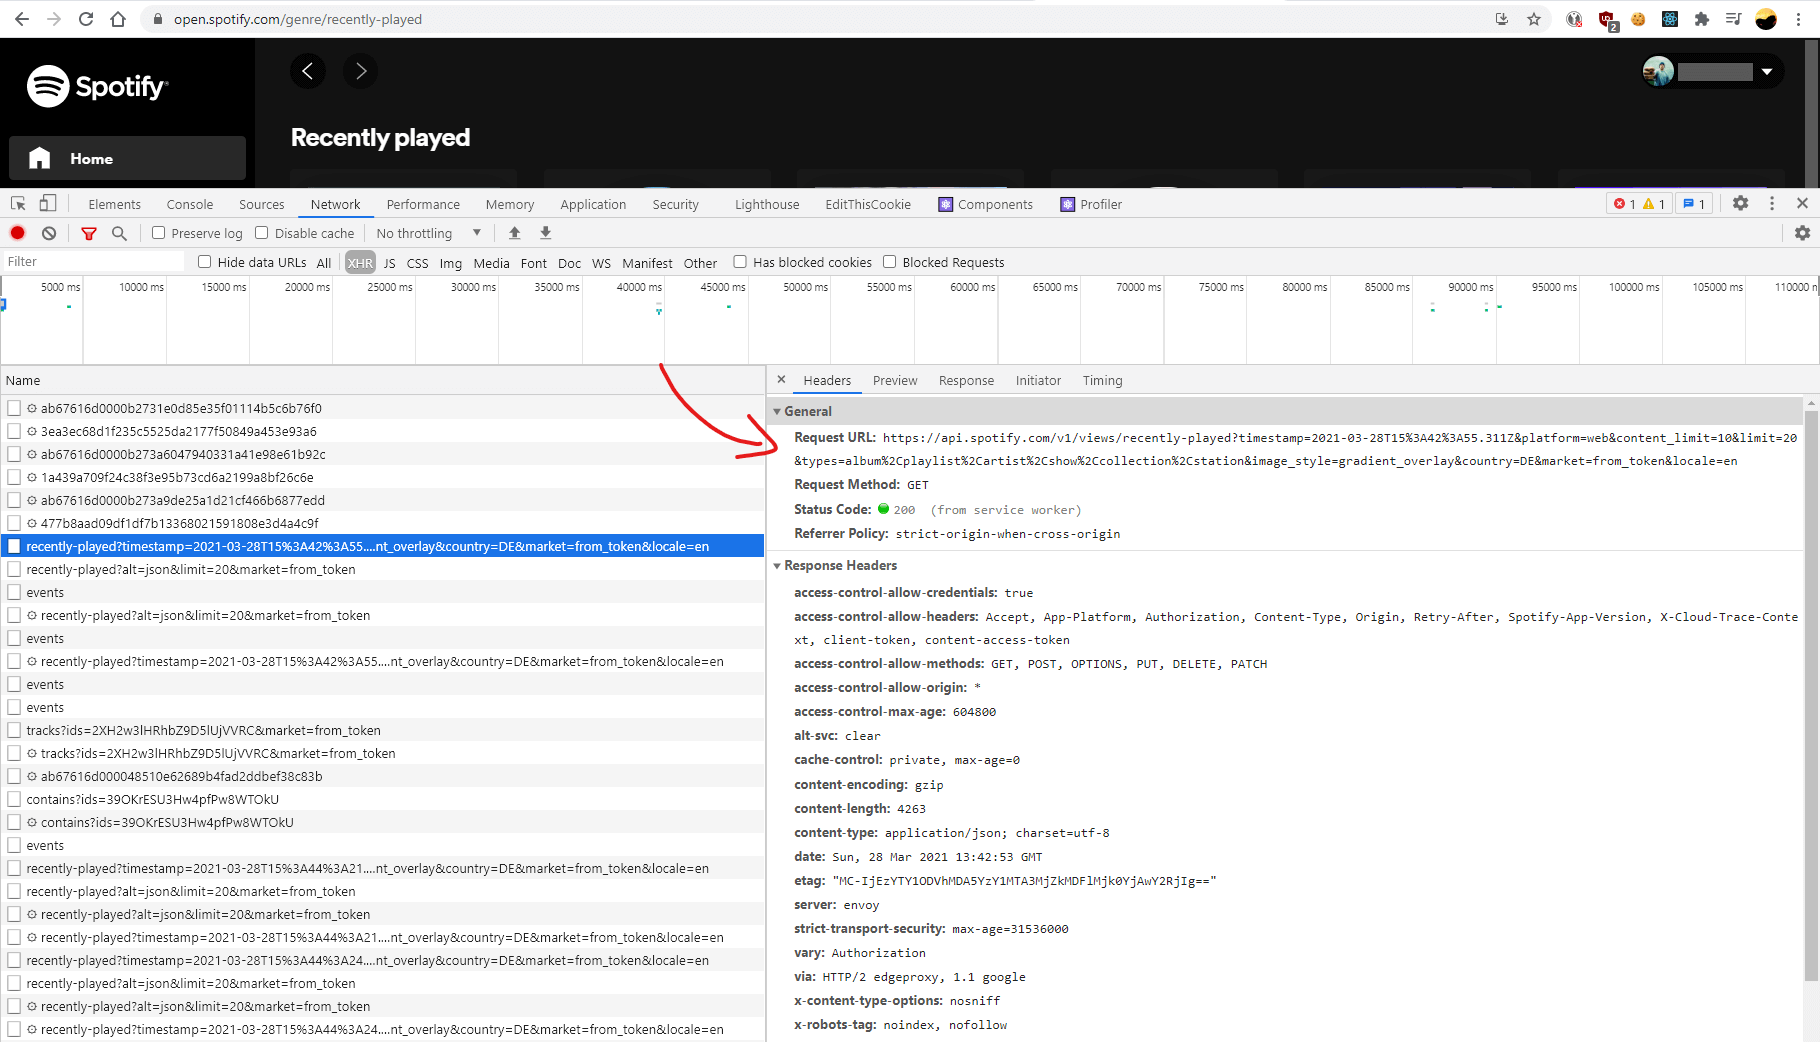
\includegraphics[width=1.0\textwidth]{Graphics/Chapter4/open-spotify-api.png}
    \caption{Spotify Web Player using different endpoints}
\end{figure}

Another issue was that we could not implement a music player with controls so you can play/pause songs or skip to the next song. Unfortunately, that functionality requires the OAuth token to be available in the frontend which implies that it does handle authentication instead of the backend. As we do server-side authentication using the backend application we had to scrap that idea and instead will open the Spotify Web Player instead. Note that the Web Playback \acs{SDK} is considered beta too \cite{SpotifyWebPlaybackSdk}.

\section{Optimizing Query Speed in PostgreSQL}

When first implementing the Jaccard algorithm using PostgreSQL functions we had query times of multiple minutes. Some of that query time was because of creating unnecessary temporary tables that get destroyed after each query. Most of the query time was because of missing query optimization though. Missing indexes made PostgreSQL scan whole tables from top to bottom which in case of the tracks tables turns out to be fatal as it contains about 66 Million rows. We fixed those two issues by creating an additional table that precomputes the lengths of playlists as well as creating some indexes.

\begin{lstlisting}[caption={Increasing query performance using a precomputed table and indexes}, style=Base, language=SQL]
    CREATE TABLE playlist_lengths AS
    SELECT COUNT(*) AS len, pid_fk
    FROM tracks
    GROUP BY pid_fk;

    CREATE INDEX ON playlist_lengths (pid_fk) INCLUDE (len);
    CREATE INDEX ON tracks (track_uri) INCLUDE (pid_fk);
    CREATE INDEX ON tracks (pid_fk) INCLUDE (track_uri);
    CREATE INDEX ON tracks (pid_fk) INCLUDE (artist_uri);
    CREATE INDEX ON tracks (pid_fk) INCLUDE (album_uri);
\end{lstlisting}

As you can see, we have created an index containing the track \ac{URI} and playlist ID. Those two fields are used to join in the Jaccard algorithm implementation. The last three indexes are used for the different variants of discover functions we have. There is a index for track, artist and album each. Using the indexes the explain graph should look like this:

\begin{figure}[bth]
    \centering
    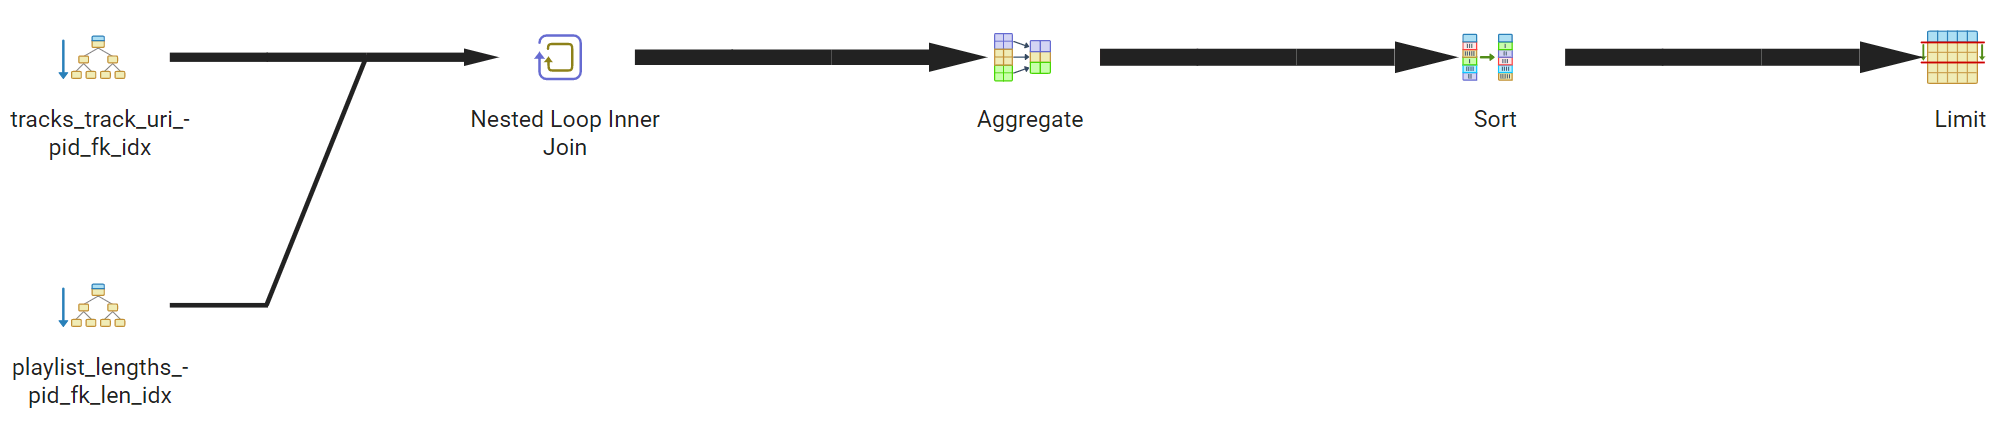
\includegraphics[width=1.0\textwidth]{Graphics/Chapter4/my-jaccard-explain.png}
    \caption{Explain graph of the my{\_}jaccard \acs{SQL} function}
\end{figure}

Looking at the textual representation of this graph shows us that PostgreSQL uses \textit{Index Only} scans instead of table scans. This approach is much faster and enables us to reduce query time to sub-second times. In case PostgreSQL still wants to use table scans, you can try running the \texttt{ANALYZE} command. In our case this was not sufficient and we had to run the \texttt{VACUUM} command so that PostgreSQL acknowledged the indexes. The command will basically do garbage-collection before running an analyze \cite{PostgresVacuum}.
